\documentclass{standalone}
\usepackage{standalone}

\begin{document}
\subsection{Burrows-Wheeler Transform (BWT)}
\subsubsection{Overview}
Burrows-Wheeler Transformation (BWT) is an interesting concept which is the basic building block of the world's one of the best indexing system called FM-index. It compresses the memory highly. Reordering the characters of a string, BWT transforms it to a more compression-friendly version. The original string could be retrieved from the transformed one through a couple of processing. The next few subsections would brief the compression procedure. A naive concept would be shown at first. Then the trade-offs would be discussed. 

\subsubsection{Burrows-Wheeler Matrix Construction}
The first step of BWT is to construct the Burrows-Wheeler Matrix (BWM) of a string. But before that, a end mark should be append to the end of the string which mark should be considered as the lowest value comparing to the any other member of the alphabet set.

\noindent Let, 

 The alphabet set, $$\sum = \{ A, T, G, C \} $$

and a string, $$S = ATTCGAGCATCAG$$

Let the endmark symbol $= \$$.
So, appending this, the string becomes, 
$$S = ATTCGAGCATCAG\$$$

The last thing to let is $ n = |S|$, where, $|\cdot|$ means the length of the string.

The matrix is $n\times n$ dimensional. To construct the matrix, $S$ should be considered as the first row. The next rows would be constructed by left shifting the characters of the $S$ in cyclic order. That means, in the last row, the end mark symbol ($\$$) would be in the first column.

In the example above, $n = 14$. So, the dimension of the matrix would be $ 14 \times 14$.

Let $S^\prime$ be the string after first cyclic left shift operation on $S$. That means, the $A$ at the beginning of the string would be removed and appended at the end of the string, after the end mark symbol. Figure \ref{fig:BWTshift} would illustrate the process better. 
$$S^\prime = TTCGAGCATCAG\$A$$

\begin{figure}
	\centering
	\tikzstyle{block} = [rectangle, draw, line width=0.5mm,
	text centered]
	\tikzstyle{line} = [draw, -latex']
	\begin{tikzpicture}[auto, node distance = 2cm]
	%first string
	\node [rectangle](lab) {$S =$};
	\node [block, dashed, anchor=west] (Val1_1) at (lab.east) {\textcolor{black!50}{A}};
	\node [block, anchor=west] (Val1_2) at (Val1_1.east) {T};
	\node [block, anchor=west] (Val1_3) at (Val1_2.east) {T};
	\node [block, anchor=west] (Val1_4) at (Val1_3.east) {C};
	\node [block, anchor=west] (Val1_5) at (Val1_4.east) {G};
	\node [block, anchor=west] (Val1_6) at (Val1_5.east) {A};
	\node [block, anchor=west] (Val1_7) at (Val1_6.east) {G};
	\node [block, anchor=west] (Val1_8) at (Val1_7.east) {C};
	\node [block, anchor=west] (Val1_9) at (Val1_8.east) {A};
	\node [block, anchor=west] (Val1_10) at (Val1_9.east) {T};
	\node [block, anchor=west] (Val1_11) at (Val1_10.east) {C};
	\node [block, anchor=west] (Val1_12) at (Val1_11.east) {A};
	\node [block, anchor=west] (Val1_13) at (Val1_12.east) {G};
	\node [block, anchor=west] (Val1_14) at (Val1_13.east) {\$};
	\node [block, anchor=west, fill=black!50] (Val1_15) at (Val1_14.east) {\textcolor{white}{A}};
	\draw[loosely dashed,line width=1mm,->] (Val1_1.north) to[bend left=20] (Val1_15.north);
	
	%second string
	\node [rectangle, below of=lab, minimum width=2cm](lab2) {$S^\prime = $};
	\node [block, anchor=west] at (lab2.east)(Val2_1) {T};
	\node [block, anchor=west] (Val2_3) at (Val2_1.east) {T};
	\node [block, anchor=west] (Val2_4) at (Val2_3.east) {C};
	\node [block, anchor=west] (Val2_5) at (Val2_4.east) {G};
	\node [block, anchor=west] (Val2_6) at (Val2_5.east) {A};
	\node [block, anchor=west] (Val2_7) at (Val2_6.east) {G};
	\node [block, anchor=west] (Val2_8) at (Val2_7.east) {C};
	\node [block, anchor=west] (Val2_9) at (Val2_8.east) {A};
	\node [block, anchor=west] (Val2_10) at (Val2_9.east) {T};
	\node [block, anchor=west] (Val2_11) at (Val2_10.east) {C};
	\node [block, anchor=west] (Val2_12) at (Val2_11.east) {A};
	\node [block, anchor=west] (Val2_13) at (Val2_12.east) {G};
	\node [block, anchor=west] (Val2_14) at (Val2_13.east) {\$};
	\node [block, anchor=west] (Val2_15) at (Val2_14.east) {A};
	\draw[line width=1.5mm,->] (Val1_8.south) to (Val2_8.north);
	\end{tikzpicture}
	\caption{Cyclic Left Shift of the First Character of  \textbf{S}. } \label{fig:BWTshift}
\end{figure}
It is the second row of the $BWM(S)$. The third row would be constructed by doing the same operation on $S^\prime$. That means the first $T$ in the above string would be moved at the end of the string, just after the character $A$.
$$S^{\prime\prime} = TCGAGCATCAG\$AT$$

In this way, other rows would be constructed. The last row would be $\$ATTCGAGCATCAG$ having the end mark symbol at the beginning as mentioned above.

Assigning the row numbers from $0$ to $n-1$, the final matrix becomes,
$$
\textbf{Pre-BWM(S)} = 
\begin{cases}
0 & ATTCGAGCATCAG\$ \\
1 & TTCGAGCATCAG\$A \\
2 & TCGAGCATCAG\$AT \\
3 & CGAGCATCAG\$ATT \\
4 & GAGCATCAG\$ATTC \\
5 & AGCATCAG\$ATTCG \\
6 & GCATCAG\$ATTCGA \\
7 & CATCAG\$ATTCGAG \\
8 & ATCAG\$ATTCGAGC \\
9 & TCAG\$ATTCGAGCA \\
10 & CAG\$ATTCGAGCAT \\
11 & AG\$ATTCGAGCATC \\
12 & G\$ATTCGAGCATCA \\
13 & \$ATTCGAGCATCAG
\end{cases}
$$
After preparing the matrix, the rows of it would be sorted lexicographically. That means, if $A$ and $B$ are two strings containing characters $A_0A_1\cdots A_{n-1}$ and $B_0B_1\cdots B_{n-1}$ respectively having same length $n$ and there exists an $i$, for which $A_i < B_i$ and $A_j = B_j$ for $0 \leq j < i < n$, then $A$ would come before $B$.

So, the sorted matrix,

$$
\textbf{BWM(S)} = 
\begin{cases}
13 & \$ATTCGAGCATCAG \\
11 & AG\$ATTCGAGCATC \\
 5 & AGCATCAG\$ATTCG \\
 8 & ATCAG\$ATTCGAGC \\
 0 & ATTCGAGCATCAG\$ \\
10 & CAG\$ATTCGAGCAT \\
 7 & CATCAG\$ATTCGAG \\
 3 & CGAGCATCAG\$ATT \\
12 & G\$ATTCGAGCATCA \\
 4 & GAGCATCAG\$ATTC \\
 6 & GCATCAG\$ATTCGA \\
 9 & TCAG\$ATTCGAGCA \\
 2 & TCGAGCATCAG\$AT \\
 1 & TTCGAGCATCAG\$A 
\end{cases}
$$
The index of the rows are preserved for certain reasons which would be discussed later. It is a clear property of the BWM that the last row of the previous matrix would go top here. 
\subsubsection{Finding BWT(S)}
Picking the last character of every string from top to bottom, a new string would be constructed which is actually the desired $BWT(S)$. To state more clearly, the above matrix could be compared with the matrix below.
$$
BWM(S)_{n,n} = 
\begin{pmatrix}
s_{1,1} & s_{1,2} & \cdots & s_{1,n} \\
s_{2,1} & s_{2,2} & \cdots & s_{2,n} \\
\vdots  & \vdots  & \ddots & \vdots  \\
s_{1,1} & s_{2,2} & \cdots & s_{n,n} 
\end{pmatrix}
$$

Taking the last character from each of the above string in matrix, $$BWT(S) = s_{1,n}s_{2,n}\cdots s_{n,n}$$

In the actual case,
$$BWT(S) = GCGC\$TGTACAATAA$$

The indexes, we saw before, are same as in Suffix Array. BWM(S) is identical to the Figure \ref{fig:suffixSort}. So, the following equation should be hold:
\[ BWT[i] =
\begin{cases}
S[ SA[i] - 1 ]       & \quad \text{if } SA[i] > 0\\
\$  & \quad \text{if } SA[i] = 0\\
\end{cases}
\]

\subsubsection{T-Ranking}
T-Ranking is not directly ranking among the whole string, rather it keeps the relative position of the same characters. To define more easily, it could be stated that the T-Ranking of a character says how many times the character is found before this position in the string. This is the condition of our string after having T-Ranking.
$$S = A_0T_0T_1C_0G_0A_1G_1C_1A_2T_2C_2A_3G_2$$
\subsubsection{LF Mapping}
LF mapping is one of the basic property of BWM. Now, by left cyclic shifting S, we could generate the BWM again. If we have only the first row and the last row of the matrix with their T-Ranking, then it is easy to find the actual string. 
$$
\textbf{BWM(S)} = 
\begin{cases}
\$\textbf{ }A_0T_0T_1C_0G_0A_1G_1C_1A_2T_2C_2A_3G_2 \\
A_3G_2\$\textbf{ }A_0T_0T_1C_0G_0A_1G_1C_1A_2T_2C_2 \\
A_1G_1C_1A_2T_2C_2A_3G_2\$\textbf{ }A_0T_0T_1C_0G_0 \\
A_2T_2C_2A_3G_2\$\textbf{ }A_0T_0T_1C_0G_0A_1G_1C_1 \\
A_0T_0T_1C_0G_0A_1G_1C_1A_2T_2C_2A_3G_2\$\textbf{ } \\
C_2A_3G_2\$\textbf{ }A_0T_0T_1C_0G_0A_1G_1C_1A_2T_2 \\
C_1A_2T_2C_2A_3G_2\$\textbf{ }A_0T_0T_1C_0G_0A_1G_1 \\
C_0G_0A_1G_1C_1A_2T_2C_2A_3G_2\$\textbf{ }A_0T_0T_1 \\
G_2\$\textbf{ }A_0T_0T_1C_0G_0A_1G_1C_1A_2T_2C_2A_3 \\
G_0A_1G_1C_1A_2T_2C_2A_3G_2\$\textbf{ }A_0T_0T_1C_0 \\
G_1C_1A_2T_2C_2A_3G_2\$\textbf{ }A_0T_0T_1C_0G_0A_1 \\
T_2C_2A_3G_2\$\textbf{ }A_0T_0T_1C_0G_0A_1G_1C_1A_2 \\
T_1C_0G_0A_1G_1C_1A_2T_2C_2A_3G_2\$\textbf{ }A_0T_0 \\
T_0T_1C_0G_0A_1G_1C_1A_2T_2C_2A_3G_2\$\textbf{ }A_0 
\end{cases}
$$

To make the think easy, the first and last columns would be kept and from this, the string could be found again. This type of keeping Last (L) and First(F) columns' data is called LF Mapping. Figure \ref{fig:LFMapping} the LF Mapping of S.
\begin{figure}
	\centering
	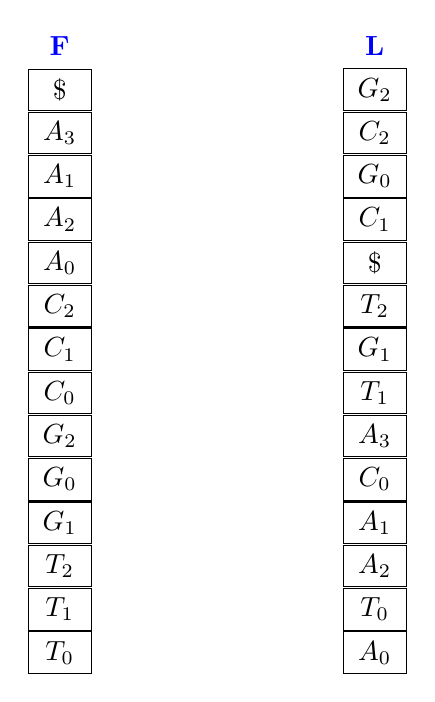
\begin{tikzpicture}[auto, node distance=5.5mm]
		% Place nodes
		\node [rectangle,color=blue,minimum width=0.8cm] (init) {\textbf{F}};
		\node [rectangle,below of=init,draw,minimum width=0.8cm] (init1) {$\$$};
		\node [rectangle,below of=init1,draw,minimum width=0.8cm] (init2) {$A_3$};
		\node [rectangle,below of=init2,draw,minimum width=0.8cm] (init3) {$A_1$};
		\node [rectangle,below of=init3,draw,minimum width=0.8cm] (init4) {$A_2$};
		\node [rectangle,below of=init4,draw,minimum width=0.8cm] (init5) {$A_0$};
		\node [rectangle,below of=init5,draw,minimum width=0.8cm] (init6) {$C_2$};
		\node [rectangle,below of=init6,draw,minimum width=0.8cm] (init7) {$C_1$};
		\node [rectangle,below of=init7,draw,minimum width=0.8cm] (init8) {$C_0$};
		\node [rectangle,below of=init8,draw,minimum width=0.8cm] (init9) {$G_2$};
		\node [rectangle,below of=init9,draw,minimum width=0.8cm] (init10) {$G_0$};
		\node [rectangle,below of=init10,draw,minimum width=0.8cm] (init111) {$G_1$};
		\node [rectangle,below of=init111,draw,minimum width=0.8cm] (init112) {$T_2$};
		\node [rectangle,below of=init112,draw,minimum width=0.8cm] (init113) {$T_1$};
		\node [rectangle,below of=init113,draw,minimum width=0.8cm] (init114) {$T_0$};
		
		\node [rectangle,color=blue,right of=init,node distance=4cm,minimum width=0.8cm] (init11) {\textbf{L}};
		\node [rectangle,below of=init11,draw,minimum width=0.8cm] (init12) {$G_2$};
		\node [rectangle,below of=init12,draw,minimum width=0.8cm] (init13) {$C_2$};
		\node [rectangle,below of=init13,draw,minimum width=0.8cm] (init14) {$G_0$};
		\node [rectangle,below of=init14,draw,minimum width=0.8cm] (init15) {$C_1$};
		\node [rectangle,below of=init15,draw,minimum width=0.8cm] (init16) {$\$$};
		\node [rectangle,below of=init16,draw,minimum width=0.8cm] (init17) {$T_2$};
		\node [rectangle,below of=init17,draw,minimum width=0.8cm] (init18) {$G_1$};
		\node [rectangle,below of=init18,draw,minimum width=0.8cm] (init19) {$T_1$};
		\node [rectangle,below of=init19,draw,minimum width=0.8cm] (init20) {$A_3$};
		\node [rectangle,below of=init20,draw,minimum width=0.8cm] (init21) {$C_0$};
		\node [rectangle,below of=init21,draw,minimum width=0.8cm] (init22) {$A_1$};
		\node [rectangle,below of=init22,draw,minimum width=0.8cm] (init23) {$A_2$};
		\node [rectangle,below of=init23,draw,minimum width=0.8cm] (init24) {$T_0$};
		\node [rectangle,below of=init24,draw,minimum width=0.8cm] (init25) {$A_0$};
	\end{tikzpicture}
	\caption{LF Mapping of the string S.}
	\label{fig:LFMapping}
\end{figure}

\subsubsection{Retrieving the string back using LF Mapping}
From the mapping in figure \ref{fig:LFMapping} the original string could be retrieved by following the steps:
\begin{enumerate}
	\item Start from the '\$' character marking as current character which is also the first character of F and take an empty string.
	\item Append the now character in previous string.
	\item Find the current character in F. and take the corresponding L as current character.
	\item Loop through until current character becomes '\$'.
	\item Reverse the string to get the original string.
\end{enumerate} 

\subsubsection{Characteristics of BWT}
There are a lot of properties of BWT, but it is here to efficiently manipulate biological genome sequences. So, here are some of the important properties of BWT:
\begin{itemize}
	\item One important properties of T-Ranking is, in both Last and First columns, the sequence of T-Ranking comes in the same order. 
	\item BWT takes very low amount of memory.
\end{itemize}
\iffalse
\tikzstyle{decision} = [diamond, draw, fill=blue!20, 
text width=4.5em, text badly centered, node distance=3cm, inner sep=0pt]
\tikzstyle{block} = [rectangle, draw, fill=blue!20, 
text width=5em, text centered, rounded corners, minimum height=4em]
\tikzstyle{line} = [draw, -latex']
\tikzstyle{cloud} = [draw, ellipse,fill=red!20, node distance=3cm,
minimum height=2em]

\begin{tikzpicture}[node distance = 2cm, auto]
% Place nodes
\node [block] (init) {initialize model};
\node [cloud, left of=init] (expert) {expert};
\node [cloud, right of=init] (system) {system};
\node [block, below of=init] (identify) {identify candidate models};
\node [block, below of=identify] (evaluate) {evaluate candidate models};
\node [block, left of=evaluate, node distance=3cm] (update) {update model};
\node [decision, below of=evaluate] (decide) {is best candidate better?};
\node [block, below of=decide, node distance=3cm] (stop) {stop};
% Draw edges
\path [line] (init) -- (identify);
\path [line] (identify) -- (evaluate);
\path [line] (evaluate) -- (decide);
\path [line] (decide) -| node [near start] {yes} (update);
\path [line] (update) |- (identify);
\path [line] (decide) -- node {no}(stop);
\path [line,dashed] (expert) -- (init);
\path [line,dashed] (system) -- (init);
\path [line,dashed] (system) |- (evaluate);
\end{tikzpicture}
\fi
\end{document}